%% ====================================================================
%% OSCM Journal — Author Template & Instructions
%% ====================================================================
%%
%%  This file is the official author guide for the Operations and
%%  Supply Chain Management (OSCM) Journal.  It doubles as a working
%%  template: replace the sample content with your own manuscript.
%%
%%  SUBMISSION WORKFLOW:
%%    - Use [preprint] for initial submission and review (single-column).
%%    - Use [review] for double-blind peer review (single-column).
%%    - Use [final] ONLY for the camera-ready version after acceptance.
%%
\documentclass[preprint]{oscmjournal}
% \documentclass[review]{oscmjournal}
% \documentclass[final]{oscmjournal}
%% ====================================================================

%% ---- Additional packages --------------------------------------------
%% The class already loads: amsmath, amssymb, bm, booktabs, multirow,
%% array, diagbox, siunitx, graphicx, xcolor, hyperref, csquotes,
%% multicol, ascmac, cuted, enumitem, caption, biblatex (APA), etc.
%%
%% Add ONLY packages the class does not provide:
\usepackage{algorithm}
\usepackage{algpseudocode}
\usepackage{amsthm}

%% ---- Theorem-like environments --------------------------------------
\newtheorem{theorem}{Theorem}
\newtheorem{proposition}[theorem]{Proposition}
\newtheorem{definition}{Definition}
\newtheorem{assumption}{Assumption}
\newtheorem{remark}{Remark}

%% ---- Bibliography ---------------------------------------------------
\addbibresource{reference.bib}

%% ---- Journal metadata (leave defaults during review) ----------------
\renewcommand{\JournalVolume}{00}
\renewcommand{\JournalNumber}{0}
\renewcommand{\JournalYear}{2026}
\renewcommand{\FirstPage}{1}
\renewcommand{\RunningHeader}{Lastname1 \& Lastname2: Author Guidelines for Preparing Manuscripts for the OSCM Journal}

%% ---- Title ----------------------------------------------------------
\title{Author Guidelines for Preparing Manuscripts for the OSCM Journal}

%% ---- Authors --------------------------------------------------------
\author[*]{Firstname1 Lastname1}
  {Affiliation, Country}
  {oscm.help@gmail.com}

  \author{Firstname2 Lastname2}
  {Affiliation, Country}
  {email@example.com}

%% ---- Keywords -------------------------------------------------------
\keywords{author guidelines, manuscript preparation, template, formatting, OSCM journal}


%% ====================================================================
\begin{document}
%% ====================================================================

\maketitle

\begin{abstract}
This document provides the official author guidelines for preparing manuscripts for the Operations and Supply Chain Management (OSCM) Journal.
It explains the submission workflow, formatting requirements, and structural expectations for each section of a paper.
The document itself is a working template: authors should replace the sample content with their own manuscript while following the guidelines described herein.
All formatting---page layout, fonts, section headings, captions, headers, and bibliography style---is handled automatically by the \LaTeX\ class file (\texttt{oscmjournal.cls}).
Authors need only provide content.
Sample elements are included throughout to illustrate how to use tables, figures, equations, theorems, algorithms, and citations within the OSCM template.
\end{abstract}


%% ====================================================================
\section{Submission Workflow}\label{sec:workflow}
%% ====================================================================

Three document class options are available, corresponding to the three stages of the publication process:

\begin{verbatim}
  \documentclass[review]{oscmjournal}
  \documentclass[preprint]{oscmjournal}
  \documentclass[final]{oscmjournal}
\end{verbatim}

The \texttt{review} option produces a single-column layout with anonymized author information (replaced by ``Anonymous Author(s)'') and hidden biographies, suitable for double-blind peer review.
The \texttt{preprint} option produces the same single-column layout but with full author names, affiliations, and biographies visible---use this for non-blind submissions or when sharing drafts with collaborators.
The \texttt{final} option produces the two-column, camera-ready layout matching the published journal format and should be used \emph{only} after formal acceptance.

Authors should not add \verb|\usepackage{}| calls for packages already loaded by the class file.
A complete list of pre-loaded packages appears at the top of \texttt{oscmjournal.cls}.


%% ====================================================================
\section{Manuscript Structure}\label{sec:structure}
%% ====================================================================

A typical OSCM manuscript follows the structure described below.
Each subsection explains what is expected and provides formatting examples using inventory management as a running illustration.

\subsection{Title, Authors, and Keywords}

The title should be concise---ideally under 20 words---and avoid abbreviations unless widely known in the OSCM community (e.g., SCM, EOQ, DEA).
Authors are listed using the \verb|\author| command, with \verb|[*]| marking the corresponding author:

\begin{verbatim}
  \author[*]{Jane Doe}
    {Industrial \& Systems Engineering Department, Sepuluh Nopember Institute of Technology, Indonesia}
    {jane.doe@its.ac.id}
  \author{John Smith}
    {School of Business, University of Example, Country}
    {john.smith@example.edu}
\end{verbatim}

Provide 3--6 keywords in lowercase, separated by commas.

\subsection{Abstract}

The abstract should be 150--250 words and state the purpose, methodology, key findings, and practical implications of the study.
Do not include citations or displayed equations in the abstract.
Where possible, include concrete numbers (e.g., ``a 20\% cost reduction'' rather than ``a significant cost reduction'').

\subsection{Introduction}

The Introduction should establish the research context, state the problem, briefly position the work relative to existing literature, identify the research gap, and summarize the paper's contributions.
Close with a road-map paragraph that outlines the remaining sections.
For example, a paper on inventory optimization might note that ``despite decades of research, many firms still set order quantities using rules of thumb'' \parencite{shee2016behavioral} and that ``recent work has highlighted the need for integrated frameworks'' \parencite{ohmori2023multi}.

\subsection{Literature Review}

Organize the literature review thematically, not chronologically.
Group related studies under descriptive subheadings.
Use \verb|\textcite{key}| for in-text citations---e.g., ``\textcite{harris1913how} introduced the EOQ model''---and \verb|\parencite{key}| for parenthetical citations---e.g., ``the bullwhip effect has been widely studied \parencite{lee1997bullwhip}.''
End the literature review with a paragraph that clearly states the research gap your paper addresses.

\subsection{Methodology}

Present your methodology with enough detail for replication.
Define notation in a table (see Table~\ref{tab:notation} for an example), number all equations you reference, and use formal environments for theorems, definitions, and proofs.
After each formal result, explain its practical or managerial implication.
If your method involves an algorithm, present it using the \texttt{algorithm} environment (see Algorithm~\ref{alg:example}).

Table~\ref{tab:notation} shows a sample notation table for an inventory study:

\begin{table}[htbp]
\tablestyle[fontsize=8, linespacing=9, stretch=1.2]
\centering
\caption{Example notation table}\label{tab:notation}
\begin{tabular*}{\columnwidth}{@{\extracolsep{\fill}}cp{\ColTableDescWidth}}
\toprule
\thead{Symbol} & \thead{Description} \\
\midrule
$D$      & Annual demand (units/year) \\
$K$      & Fixed ordering cost (\$/order) \\
$h$      & Holding cost (\$/unit/year) \\
$Q^*$    & Optimal order quantity (units) \\
\bottomrule
\end{tabular*}
\end{table}

The following equation illustrates how to present the classic EOQ total cost function.
Equations should be numbered when referenced in the text:
\begin{equation}
\text{TC}(Q) = \frac{D}{Q}\,K + \frac{Q}{2}\,h \label{eq:totalcost}
\end{equation}

Minimizing Eq.~\eqref{eq:totalcost} yields the well-known EOQ formula \parencite{harris1913how}:

\begin{theorem}[Optimal EOQ]\label{thm:eoq}
The order quantity minimizing $\mathrm{TC}(Q)$ is $Q^* = \sqrt{2DK/h}$.
\end{theorem}

\begin{proof}
Setting $d\,\text{TC}/dQ = 0$ gives $Q^* = \sqrt{2DK/h}$; the positive second derivative confirms a minimum.
\end{proof}

\begin{remark}\label{rem:sqrtcost}
The optimal cost $\sqrt{2DKh}$ grows with the square root of demand, meaning a warehouse with twice the demand needs only 41\% more budget. This insight supports demand-consolidation strategies.
\end{remark}

Authors may also use definitions to introduce key concepts, and assumptions to state modeling conditions:

\begin{definition}[Critical Ratio]\label{def:cr}
The critical ratio balances the cost of understocking ($c_u = p - c$) against overstocking ($c_o = c - v$):
$\text{CR} = {c_u}/({c_u + c_o}) = ({p - c})/({p - v})$.
\end{definition}

\begin{assumption}\label{asm:normal}
Demand during lead time $L$ is normally distributed with mean $DL/52$ and variance $\sigma_D^2 L$.
\end{assumption}

When a proof is long or technical, state the result in the main text and defer the proof to the appendix.
Theorem~\ref{thm:newsvendor} illustrates this pattern:

\begin{theorem}[Optimal Newsvendor Quantity]\label{thm:newsvendor}
Under Assumption~\ref{asm:normal}, the profit-maximizing order quantity satisfies $F(Q^*) = (p-c)/(p-v)$, where $F(\cdot)$ is the CDF of demand.
\end{theorem}

The proof of Theorem~\ref{thm:newsvendor} is given in Appendix~\ref{app:proofs}.
This approach keeps the main text focused on results and their managerial implications---for instance, the critical ratio (Definition~\ref{def:cr}) tells managers that when margins are high relative to markdown losses, they should order aggressively.

Algorithm~\ref{alg:example} shows how to present pseudocode:

\begin{algorithm}[htbp]
\caption{Example: $(Q, R)$ Policy Optimization}\label{alg:example}
\begin{algorithmic}[1]
\Require $D$, $K$, $h$, $L$, $\sigma_D$, $\alpha$
\Ensure $Q^*$, $R^*$
\State $Q \leftarrow \sqrt{2DK / h}$
\Repeat
    \State Update $R$ based on service level $\alpha$
    \State Update $Q$ incorporating shortage cost
\Until{convergence}
\State $Q^* \leftarrow Q$,\; $R^* \leftarrow R$
\end{algorithmic}
\end{algorithm}


\subsection{Results and Discussion}

Present results using well-formatted tables and figures.
Always discuss your results---do not merely present numbers.
Relate findings back to the research questions posed in the Introduction and draw out the managerial implications.

Use single-column tables (\verb|\begin{table}|) for narrow data and full-width tables (\verb|\begin{table*}|) for wider data.
Table~\ref{tab:example_results} illustrates a single-column results table, and Table~\ref{tab:example_wide} illustrates a full-width table.

\begin{table}[htbp]
\tablestyle[fontsize=8, linespacing=9, stretch=1.3]
\centering
\caption{Example results table (single-column)}\label{tab:example_results}
\begin{tabular*}{\columnwidth}{@{\extracolsep{\fill}}lSSS}
\toprule
\thead{Region} & {$D$ (units/yr)} & {$Q^*$ (units)} & {\thead{TC (\$/yr)}} \\
\midrule
North America  & 12000 & 490  & 4900 \\
Europe         & 8500  & 412  & 4120 \\
East Asia      & 15000 & 548  & 5480 \\
\bottomrule
\end{tabular*}
\begin{flushleft}
\footnotesize \textit{Notes}: Use footnotes to explain abbreviations.
\end{flushleft}
\end{table}

\begin{table*}[htbp]
\tablestyle[fontsize=8, linespacing=9, stretch=1.2, colsep=8pt]
\centering
\caption{Example sensitivity analysis (full-width table)}\label{tab:example_wide}
\begin{tabular*}{\textwidth}{@{\extracolsep{\fill}}lSSSSS}
\toprule
\thead{Region} & {$K{-}20\%$} & {$K{-}10\%$} & {\thead{Baseline}} & {$K{+}10\%$} & {$K{+}20\%$} \\
\midrule
North America  & 4380 & 4640 & 4900 & 5150 & 5390 \\
Europe         & 3690 & 3900 & 4120 & 4330 & 4530 \\
East Asia      & 4900 & 5190 & 5480 & 5760 & 6030 \\
\bottomrule
\end{tabular*}
\begin{flushleft}
\footnotesize \textit{Notes}: All values in \$/year.
\end{flushleft}
\end{table*}

For figures, use vector formats (PDF, EPS) whenever possible.
Pre-compile TikZ or matplotlib figures to PDF and include them with \verb|\includegraphics|.
Figure~\ref{fig:example} demonstrates this approach.
Use \verb|\begin{figure}| for single-column and \verb|\begin{figure*}| for full-width figures.
Every figure and table must be referenced in the text.

\begin{figure}[htbp]
\centering
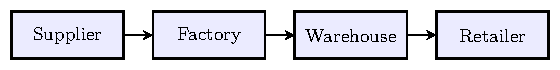
\includegraphics[width=0.7\columnwidth]{figs/supply-chain.pdf}
\caption{Example figure: a four-echelon supply chain}\label{fig:example}
\end{figure}


\subsection{Conclusion and Future Research}

The conclusion should summarize the paper's contributions without repeating the abstract, state practical implications for managers and practitioners, acknowledge limitations honestly, and suggest concrete directions for future research.


%% ====================================================================
\section{Formatting Details}\label{sec:formatting}
%% ====================================================================

This section covers additional formatting requirements.

\subsection{Citations and References}

OSCM uses APA citation style, handled automatically by the class file via \texttt{biblatex}.
Store your references in a \texttt{.bib} file and declare it with \verb|\addbibresource{references.bib}|.
Use \verb|\textcite{key}| for ``Author (Year)'' in running text: for example, \textcite{zipkin2000foundations} provides a comprehensive treatment of inventory theory.
Use \verb|\parencite{key}| for parenthetical citations: coordination contracts can improve supply chain performance \parencite{nandi2016dynamics}.
For multiple citations: \verb|\parencite{key1, key2}| produces \parencite{cachon2000supply, lee1997bullwhip}.

\subsection{Tables}

Use booktabs rules (\verb|\toprule|, \verb|\midrule|, \verb|\bottomrule|) instead of vertical lines.
The \verb|\tablestyle[...]| command lets you override font size, line spacing, row stretch, and column separation on a per-table basis.
Use \verb|\thead{...}| for bold column headers.
Place table notes in a \verb|\begin{flushleft}...\end{flushleft}| block below the table.

\subsection{Equations}

Number all equations referenced in the text using the \texttt{equation} or \texttt{align} environments.
Reference them with \verb|\eqref{label}|: ``as shown in Eq.~\eqref{eq:totalcost}.''
For multi-line equations, use \texttt{align} and align on the relation symbol.

\subsection{Figures}

Figures should be at least 300 dpi for rasterized images or in vector format (PDF preferred).
Center all figures and provide descriptive captions.

\subsection{Theorems, Proofs, and Algorithms}

Use \verb|\begin{theorem}|, \verb|\begin{definition}|, \verb|\begin{proof}|, etc.\ for formal results.
The class does not pre-define these environments, so declare them in the preamble as shown at the top of this file.
After each theorem or proposition, explain its managerial significance (see Remark~\ref{rem:sqrtcost} for an example).
Use the \texttt{algorithm} and \texttt{algpseudocode} packages for pseudocode (see Algorithm~\ref{alg:example}).

\subsection{Acknowledgements}

Use a section (\verb|\section*{Acknowledgements}|) to acknowledge funding sources, data providers, and colleagues who contributed but do not meet authorship criteria.


%% ====================================================================
\section*{Acknowledgements}
%% ====================================================================

The OSCM Editorial Office thanks the journal's reviewers, editors, and advisory board for their ongoing contributions to maintaining the quality and relevance of the journal.


%% ====================================================================
\printbibliography[title={REFERENCES}]


%% ====================================================================
%% BIOGRAPHIES
%% ====================================================================

\begin{strip}
\biographies
\vspace{1em}

\begin{biography}{First A. Author}
(PhD) is an Associate Professor in the Department of Industrial Engineering at the University of Example, Country.
She received her PhD in Operations Research from Top University in 2015.
Her research interests include supply chain optimization, inventory management, and sustainable operations.
\end{biography}
\vspace{1em}

\begin{biography}{Second B. Author}
(PhD) is a Professor in the School of Business at Another University, Country.
He received his PhD in Management Science from Leading University in 2008.
His research focuses on production planning, supply chain coordination, and stochastic modeling.
\end{biography}
\vspace{1em}

\begin{biography}{Third C. Author}
(PhD) is an Assistant Professor in the Faculty of Engineering at Yet Another University, Country.
He received his PhD in Industrial Engineering from Research University in 2020.
His research interests lie in logistics network design and humanitarian operations.
\end{biography}
\end{strip}


%% ====================================================================
%% APPENDIX
%% ====================================================================

~ %needed to avoid the page break

\onecolumn
\appendix
\section{Appendix}

\subsection{Example Appendix Table}

Table~\ref{tab:appdata} illustrates how to present supplementary data in the appendix.

\begin{table*}[htbp]
\tablestyle[fontsize=8, linespacing=9, stretch=1.2, colsep=8pt]
\centering
\caption{Example input data by region (appendix table)}\label{tab:appdata}
\begin{tabular*}{\textwidth}{@{\extracolsep{\fill}}lSSSSS}
\toprule
\thead{Parameter} & {\thead{N.\ America}} & {\thead{Europe}} & {\thead{E.\ Asia}} & {\thead{SE Asia}} & {\thead{S.\ America}} \\
\midrule
Annual demand (units/yr)       & 12000 & 8500  & 15000 & 6000 & 4200 \\
Ordering cost (\$/order)       & 100   & 110   & 95    & 85   & 105  \\
Holding cost (\$/unit/yr)      & 5.00  & 5.50  & 4.75  & 4.25 & 5.25 \\
Lead time (weeks)              & 2     & 3     & 1     & 2    & 4    \\
\bottomrule
\end{tabular*}
\end{table*}

\subsection{Proofs}\label{app:proofs}

Authors may defer lengthy proofs to the appendix to keep the main text readable.
Reference the appendix from the main text (e.g., ``the proof is given in Appendix~\ref{app:proofs}'').

\begin{proof}[Proof of Theorem~\ref{thm:newsvendor}]
The expected profit when ordering $Q$ units is:
\begin{equation}
\Pi(Q) = (p - c)\,E[\min(D, Q)] - (c - v)\,E[\max(Q - D, 0)] \label{eq:nv_profit}
\end{equation}
Differentiating with respect to $Q$:
\begin{align}
\frac{d\Pi}{dQ} &= (p - c)\bigl(1 - F(Q)\bigr) - (c - v)\,F(Q) \nonumber \\
                &= (p - c) - (p - v)\,F(Q) \label{eq:nv_deriv}
\end{align}
Setting Eq.~\eqref{eq:nv_deriv} to zero and solving for $F(Q)$ yields:
\begin{equation}
F(Q^*) = \frac{p - c}{p - v} \label{eq:nv_solution}
\end{equation}
The second derivative $\frac{d^2\Pi}{dQ^2} = -(p-v)\,f(Q) < 0$ confirms that $Q^*$ is a maximum.
\end{proof}


\subsection{Example Appendix Derivation}

Authors may also place extended model derivations here.
For instance, extending the EOQ (Theorem~\ref{thm:eoq}) to planned shortages with backorder cost $b$ yields:
\begin{equation}
Q^* = \sqrt{\frac{2DK}{h}} \cdot \sqrt{\frac{h + b}{b}} \label{eq:eoq_short}
\end{equation}
When $b \to \infty$, Eq.~\eqref{eq:eoq_short} reduces to the standard EOQ, confirming internal consistency.

\end{document}
